\PassOptionsToPackage{table}{xcolor}
\documentclass[aspectratio=169]{beamer}\usepackage[utf8]{inputenc}
\usepackage{lmodern}
\usepackage[english]{babel}
\usepackage{color}
\usepackage{amsmath,mathtools}
\usepackage{booktabs}
\usepackage{mathptmx}
\usepackage[11pt]{moresize}
\usepackage{hyperref}
\usepackage{commath}
\usepackage{bm}
\usepackage{subfigure}
\usepackage{siunitx}
\usepackage{multirow}

\usepackage{listings}
\definecolor{mygreen}{RGB}{28,172,0}
\definecolor{mylilas}{RGB}{170,55,241}

\setbeamertemplate{navigation symbols}{}
\setbeamersize{text margin left=5mm,text margin right=5mm}
\setbeamertemplate{caption}[numbered]
\addtobeamertemplate{navigation symbols}{}{
\usebeamerfont{footline}
\usebeamercolor[fg]{footline}
\hspace{1em}
\insertframenumber/\inserttotalframenumber}

\newcommand{\R}{\mathbb{R}}
\newcommand{\E}{\mathbb{E}}
\newcommand{\N}{\mathbb{N}}
\newcommand{\Z}{\mathbb{Z}}
\newcommand{\V}{\mathbb{V}}
\newcommand{\Q}{\mathbb{Q}}
\newcommand{\K}{\mathbb{K}}
\newcommand{\C}{\mathbb{C}}
\newcommand{\T}{\mathbb{T}}
\newcommand{\I}{\mathbb{I}}

\title{MATLAB: Read Me}
\subtitle{Renzo Miguel Caballero Rosas}

\begin{document}

\lstset{language=Matlab,
    breaklines=true,
    morekeywords={matlab2tikz},
    keywordstyle=\color{blue},
    morekeywords=[2]{1}, keywordstyle=[2]{\color{black}},
    identifierstyle=\color{black},
    stringstyle=\color{mylilas},
    commentstyle=\color{mygreen},
    showstringspaces=false,
    numbers=left,%
    numberstyle={\tiny \color{black}},
    numbersep=9pt,
    emph=[1]{for,end,break},emphstyle=[1]\color{red},  
}

\begin{frame}
\titlepage
\end{frame}


\setbeamercolor{background canvas}{bg=white!10}
\begin{frame}\frametitle{Code diagram:}

\begin{figure}[ht!]
\centering
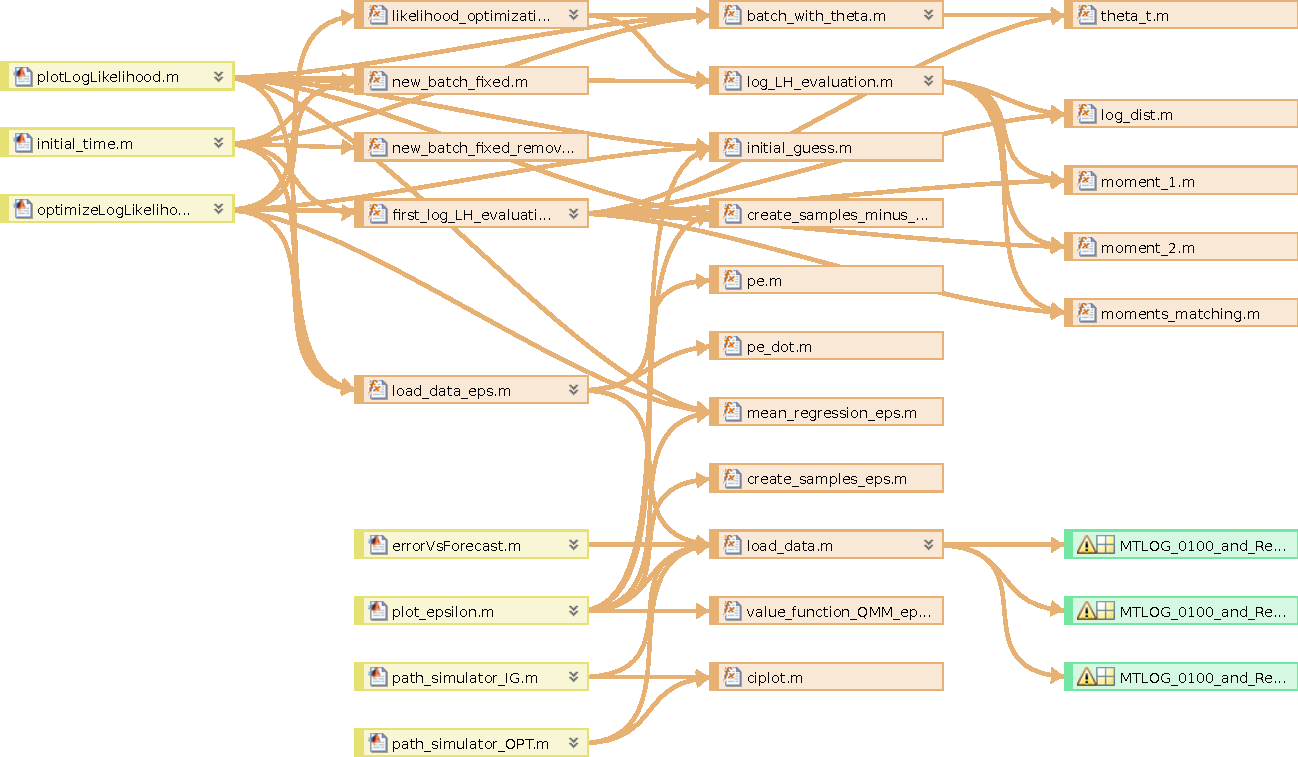
\includegraphics[width=0.8\textwidth]{../Results/project/20200320_MATLAB_Files_Graph.pdf}
\end{figure}

\end{frame}


\setbeamercolor{background canvas}{bg=white!10}
\begin{frame}\frametitle{Questions:}

\begin{itemize}

\item Why $\dif X=a(X;\alert{\theta})\dif t+b(X;\alert{\theta},\alert{\alpha})\dif W$ and no $\dif X=a(X;\alert{\theta})\dif t+b(X;\alert{\gamma})\dif W$? Where all $\alert{\theta},\alert{\alpha},\alert{\gamma}\in\R^+$. {\color{green}Because in the way it is defined, $\theta$ controls the mean reversion and $\alpha$ the wide of the confidence band.} {\color{red} However, maybe it is better to optimize over $\theta$ and $\gamma$? Because of the relative dimension. After, trivially we can compute $\alpha=\gamma/\theta$}.

\item Which is Beta, the measurements or the transitions? 

\item Which data in the histograms? Measurements or transitions? 

\end{itemize}

\end{frame}


\setbeamercolor{background canvas}{bg=white!10}
\begin{frame}\frametitle{Some keywords:}

\begin{itemize}

\item Our process is: \textbf{High-frequency in a fixed time-interval}.

\end{itemize}

\end{frame}


\setbeamercolor{background canvas}{bg=white!10}
\begin{frame}\frametitle{Normalization:}\label{Norm}

Given the SDE
\begin{equation*}
\dif V_t=-\theta_tV_t\dif t+\sqrt{2\theta_0\alpha(V_t+p_t)(1-V_t-p_t)}\dif W_t,
\end{equation*}
we consider the normalized differentials $\dif\hat{t}=\frac{\dif t}{T}$, and $\dif\hat{W}_t=\frac{\dif W_t}{\sqrt{T}}$. Then, we can write the SDE as
\begin{equation*}
\dif V_t=-\alert{\theta_tT}V_t\dif\hat{t}+\sqrt{2\alert{\theta_0T}\alpha(V_t+p_t)(1-V_t-p_t)}\dif\hat{W}_t.
\end{equation*}
We conclude that, whatever the normalization constant T is, it gets absorbed by the parameter $\theta_t$ or $\theta_0$ (let $\hat{\theta}_t=\theta_t T$ and $\hat{\theta}_0=\theta_0 T$).
\quad\\
The E-M representation is
\begin{equation*}
V_{t_{n+1}}=V_{t_{n}}-\left[\hat{\theta}_{t_n}V_{t_n}\right]\Delta s+\left[\sqrt{2\hat{\theta}_{0}\alpha(V_{t_n}+p_{t_n})(1-V_{t_n}-p_{t_n})}\right]\sqrt{\Delta s}\Delta\hat{W}_{t_n},\ V_{t_0}=v_0,
\end{equation*}
for $n\in\{0\dots,m-1\}$, $t_j=t_0+j\Delta s$, $t_0=0$, $t_m=1$, and $\Delta\hat{W}_{t_n}$ normal (0,1) for each $t_n$.

\end{frame}


\setbeamercolor{background canvas}{bg=white!10}
\begin{frame}\frametitle{SDE first moment (1/2):} \label{m1}
Given some measurement $v_{t_{n-1}}$, we want to compute the first moment at time $t_n$. The exact first moment $m_1(s)$ for $s\in[t_{n-1},t_n]$ is the solution of the ODE

\begin{equation*}
\begin{cases}
\dif m_1(s)=\left[-m_1(s)\theta(s)\right]\dif s,\\
m_1(t_{n-1})=v_{t_{n-1}}.
\end{cases}
\end{equation*}
If $\theta(t_{n-1})=\theta(t_{n})=\theta$, the solution is $m_1(t_n)=m_1(t_{n-1})e^{-\theta(t_n-t_{n-1})}$.\\
\quad\\
Otherwise, we compute a linear interpolation for $\theta(s)$ and solve the ODE using Forward-Euler:
\begin{equation*}
m_1(s_{n})=m_1(s_{n-1})(1-\theta(s_{n-1})\Delta s).
\end{equation*}

\end{frame}


\setbeamercolor{background canvas}{bg=white!10}
\begin{frame}\frametitle{SDE first moment (2/2): CODE} \label{m1_code}

\begin{center}
\begin{tabular}{|c|}
\toprule
{\footnotesize
\lstinputlisting{../moment_1.m}
}\\
\bottomrule
\end{tabular}
\end{center}

\end{frame}


\setbeamercolor{background canvas}{bg=white!10}
\begin{frame}\frametitle{SDE second moment (1/2):} \label{m2}

Given some measurement $v_{t_{n-1}}$, we want to compute the second moment at time $t_n$. The exact second moment $m_2(s)$ for $s\in[t_{n-1},t_n]$ is the solution of the ODE

\begin{equation*}
\begin{cases}
\dif m_2(s)&=\left[\alert{-2m_2(s)(\theta(s)+\alpha\theta_0)}+2\alpha\theta_0m_1(s)(1-2p(s))+{\color{blue}2\alpha\theta_0p(s)(1-p(s))}\right]\dif s,\\
m_2(t_{n-1})&=v^2_{t_{n-1}}.
\end{cases}
\end{equation*}
We compute a linear interpolation for the functions $\theta(s)$ and $p(s)$. After, we solve the ODE using Forward-Euler:
{\scriptsize
\begin{equation*}
m_2(s_n)=m_2(s_{n-1})+\left[\alert{-2m_2(s_{n-1})(\theta(s_{n-1})+\alpha\theta_0)}+2\alpha\theta_0m_1(s_{n-1})(1-2p(s_{n-1}))+{\color{blue}2\alpha\theta_0p(s_{n-1})(1-p(s_{n-1}))}\right]\Delta s.
\end{equation*}}
We use the same discretization points for both $m_1(s)$ and $m_2(s)$.

\end{frame}


\setbeamercolor{background canvas}{bg=white!10}
\begin{frame}\frametitle{SDE second moment (2/2): CODE} \label{m2_code}

\begin{center}
\begin{tabular}{|c|}
\toprule
{\tiny
\lstinputlisting{../moment_2.m}
}\\
\bottomrule
\end{tabular}
\end{center}

\end{frame}


\setbeamercolor{background canvas}{bg=white!10}
\begin{frame}\frametitle{Density next measurement (1/2):} \label{Tr}

We want the next measurement $V_{t_n}|V_{t_{n-1}}$ to have a Beta distribution, but with support in $[a,b]=[-1,1]$. Given $X\sim\beta(\xi_1,\xi_2)$ a \alert{Beta distributed random variable}, we define the new random variable $V=a+(b-a)X$ with support in $[-1,1]$, and PDF $f_V(v)$.\\
\quad\\
We can compute:
\begin{itemize}
\item $\E[V]=a+(b-a)\E[X]=a+(b-a)\frac{\xi_1}{\xi_1+\xi_2}=\mu_V$.
\item $\V[V]=(b-a)^2\V[X]=\frac{(b-a)^2\xi_1\xi_2}{(\xi_1+\xi_2)^2(\xi_1+\xi_2+1)}=\sigma^2_V$.
\end{itemize}
\quad\\
\quad\\
Then, we want the SDE and our new PDF $f_V(v)$ to have the same moments at each $t\in\{\text{some appropriate domain}\}$, i.e., $\mu(t)=m_1(t)$ and $\sigma^2(t)=m_2(t)-m_1^2(t)$.\\
$\mu(t)$ and $\sigma^2(t)$ refers to the mean and variance of $V_{t_n}|V_{t_{n-1}}$, following the structure described for $f_V(v)$.

\end{frame}


\setbeamercolor{background canvas}{bg=white!10}
\begin{frame}\frametitle{Density next measurement (2/2):}

For each measurement $V_{t_{n-1}}$, we can find the analytical moments for the SDE at time $t_n$ solving the ODEs from slides {\color{blue}\ref{m1}} and {\color{blue}\ref{m2}}. Then, we can find the parameters $\xi_1$ and $\xi_2$ such that both the SDE and the PDF of $V_{t_n}|V_{t_{n-1}}$ have the same first and second moments at time $t_n$.
\begin{itemize}
\item $\xi_1=-\frac{(1+\mu)(\mu^2+\sigma^2-1)}{2\sigma^2}$ all evaluated at time $t_n$ (verified in \textbf{Mathematica 11.0}\footnote{File: {\color{blue}matchingVerification.nb}.}).
\item $\xi_2=\frac{(\mu-1)(\mu^2+\sigma^2-1)}{2\sigma^2}$ all evaluated at time $t_n$ (verified in \textbf{Mathematica 11.0}).
\end{itemize}

\begin{center}
\begin{tabular}{|c|}
\toprule
{\footnotesize
\lstinputlisting{../moments_matching.m}
}\\
\bottomrule
\end{tabular}
\end{center}

\end{frame}


\setbeamercolor{background canvas}{bg=white!10}
\begin{frame}\frametitle{Log-density (1/2):}

Recall the PDF $f_V(v)$ from slide {\color{blue}\ref{Tr}}. We will use this density to model the random variables $V_{t_n}|V_{t_{n-1}}$. For $[a,b]=[-1,1]$, we have that
\begin{equation*}
f_V(v)=f_X(g^{-1}(v))\left|\frac{\dif}{\dif v}g^{-1}(v)\right|\quad \text{where}\quad f_X(x)=\text{Beta}(\xi_1,\xi_2)\quad\text{and}\quad g(x)=a+(b-a)x.
\end{equation*}
Then, $f_V(v)=\frac{1}{|(b-a)|}\frac{1}{B(\xi_1,\xi_2)}\left(\frac{v-a}{b-a}\right)^{\xi_1-1}\left(1-\frac{v-a}{b-a}\right)^{\xi_2-1}$ because $g^{-1}(v)=\frac{v-a}{b-a}$.\\
\quad\\
Also, we have that (up to some constant values)
\begin{equation*}
\log\left(f_V(v)\right)=\log\left(\frac{1}{B(\xi_1,\xi_2)}\right)+(\xi_1-1)\log\left(\frac{v-a}{b-a}\right)+(\xi_2-1)\log\left(\frac{b-v}{b-a}\right),
\end{equation*}
where $\xi_1$ and $\xi_2$ depends on the SDE moments.

\end{frame}


\setbeamercolor{background canvas}{bg=white!10}
\begin{frame}\frametitle{Log-density (2/2): CODE}

\begin{center}
\begin{tabular}{|c|}
\toprule
{\footnotesize
\lstinputlisting{../log_dist.m}
}\\
\bottomrule
\end{tabular}
\end{center}
Notice we use the function \textbf{betaln(a,b)}. It is important to compute the log directly for the beta function, and no first the beta, and after apply log.
\end{frame}


\setbeamercolor{background canvas}{bg=white!10}
\begin{frame}\frametitle{Log-likelihood (1/2):}

We introduce the number of paths $M$, and the number of measurements per path $N+1$ ($N$ transitions). Then, we have a total of $M\times N$ samples to use. Notice that each pair $(\xi_1,\xi_2)$ depends on $i\in\{1,\dots,M\}$ and $j\in\{2,\dots,N+1\}$. Then, the log-likelihood is
\begin{equation*}
\mathfrak{L}\left(\{V\}_{M,N}\right)=\sum_{i=1}^M\sum_{j=2}^{N+1}\log\left[\rho_{i,j}\left(V_{i,j}|V_{i,j-1}\right)\right],
\end{equation*}
where $\rho_{i,j}\left(V_{i,j}|V_{i,j-1}\right)=\rho_{i,j}\left(V_{i,j}|V_{i,j-1};\xi_{1_{i,j}},\xi_{2_{i,j}}\right)$, and where we assumed a non-informative prior.

\end{frame}


\setbeamercolor{background canvas}{bg=white!10}
\begin{frame}\frametitle{Data: CODE}

We load our three tables: \textbf{Table\_Training\_Complete}, \textbf{Table\_Testing\_Complete}, and \textbf{Table\_Complete}.

\begin{center}
\begin{tabular}{|c|}
\toprule
{\tiny
\lstinputlisting{../load_data.m}
}\\
\bottomrule
\end{tabular}
\end{center}

\end{frame}


\setbeamercolor{background canvas}{bg=white!10}
\begin{frame}\frametitle{From $\theta_0$ to $\theta_t$:}

To ensure that the analytical solutions is always in $]0,1[$, we choose the drift parameter to be
\begin{equation*}
\theta(t) = \max\left(\theta_0,\frac{\theta_0\alpha+|\dot{p}^\epsilon(t)|}{\min(p^\epsilon(t),1-p^\epsilon(t))}\right),\quad\theta_0>0.
\end{equation*}
\quad\\
\quad\\
\begin{center}
\begin{tabular}{|c|}
\toprule
{\tiny
\lstinputlisting{../theta_t.m}
}\\
\bottomrule
\end{tabular}
\end{center}
{\tiny Recall that we normalized w.r.t. time $T$. The normalized $\hat{\theta}_t$ is $\hat{\theta}_t=\theta_tT$. Notice that in the definition of $\theta_t$, if we use $\hat{\theta}_0=\theta_0T$ and the derivative of $p_t$ w.r.t. $\dif \hat{t}$ instead of w.r.t. $\dif t$, then we automatically have $\hat{\theta}_t$. See slide \ref{Norm}.}

\end{frame}


\setbeamercolor{background canvas}{bg=white!10}
\begin{frame}\frametitle{From $p_t$ to $p_t^\epsilon$:}

To ensure that $\theta(t)$ does not blow up, we truncate the forecast so it is always in $[\epsilon,1-\epsilon]$ for some $\epsilon\in(0,1/2)$.

{\small
\begin{columns}[c]

\column{.5\textwidth}
Where $p^\epsilon(t)=\begin{cases}
\epsilon\quad&\text{if}\quad p(t)<\epsilon\\
p(t)\quad&\text{if}\quad \epsilon\leq p(t)<1-\epsilon\\
1-\epsilon\quad&\text{if}\quad p(t)\geq1-\epsilon
\end{cases}$.

\column{.5\textwidth}
\begin{center}
\begin{tabular}{|c|}
\toprule
{\tiny
\lstinputlisting{../pe.m}
}\\
\bottomrule
\end{tabular}
\end{center}

\end{columns}}

{\small
\begin{columns}[c]

\column{.5\textwidth}
$\dot{p}^\epsilon_t=\frac{\dif p^\epsilon}{\dif t}$. We use finite differences.

\column{.5\textwidth}
\begin{center}
\begin{tabular}{|c|}
\toprule
{\tiny
\lstinputlisting{../pe_dot.m}
}\\
\bottomrule
\end{tabular}
\end{center}

\end{columns}}

\end{frame}


\setbeamercolor{background canvas}{bg=white!10}
\begin{frame}\frametitle{Adapting the data:}

\begin{columns}[c]

\column{.2\textwidth}
We use this function to truncate the forecast, calculate its derivative, and to define the new errors ($X_t-p_t^\epsilon$) associated with the new truncated forecast.\\
We call to all this new set of data, the truncated data.

\column{.7\textwidth}
\begin{center}
\begin{tabular}{|c|}
\toprule
{\tiny
\lstinputlisting{../load_data_eps.m}
}\\
\bottomrule
\end{tabular}
\end{center}

\end{columns}

\end{frame}


\setbeamercolor{background canvas}{bg=white!10}
\begin{frame}\frametitle{Create a new batch (1/2):} \label{cre_batch}

\alert{This function is independent of if we are using the real data or the truncated one.}\\
If we take a total of $Z\in\N$ days, the batch corresponding to this days is
\begin{table}[]
\begin{tabular}{|c|c|c|c|c|c|c|c|c|}
\hline
\multicolumn{7}{|l|}{PATH 1}                                                                                       & ...                  & PATH Z               \\ \hline
\multicolumn{2}{|l|}{$t_n=01:10$}   & \multicolumn{2}{l|}{$t_n=01:20$}    & ... & \multicolumn{2}{l|}{$t_n=00:50$} & \multirow{4}{*}{...} & \multirow{4}{*}{...} \\ \cline{1-7}
$p(t_{n-1})$      & $p(t_{n})$      & $p(t_{n-1})$      & $p(t_{n})$      & ... & $p(t_{n-1})$     & $p(t_{n})$    &                      &                      \\ \cline{1-7}
$\dot{p}(t_{n-1})$ & $\dot{p}(t_{n})$ & $\dot{p}(t_{n-1})$ & $\dot{p}(t_{n})$ & ... & $\dot{p}(t_{n-1})$     & $\dot{p}(t_{n})$    &                      &                      \\ \cline{1-7}

$V(t_{n-1})$      & $V(t_{n})$      & $V(t_{n-1})$      & $V(t_{n})$      & ... & $V(t_{n-1})$     & $V(t_{n})$    &                      &                      \\ \hline
\end{tabular}
\end{table}
with dimensions $3\times(2Z(N-1))$. As an example: If we have 145 measurements (N+1), then $N=144$ and $N-1=143$. We use 143 samples because we need to ignore the initial measurement (because we do not have data at time $t_{-1}$) and the final one (because it does not have $\dot{p}$). Then, each day has 143 samples. In this implementation, we are duplicating the data. In case of a lack of RAM, we can reduce the dimensions to $3\times(Z(N-1))$.
\end{frame}


\setbeamercolor{background canvas}{bg=white!10}
\begin{frame}\frametitle{Create a new batch (2/2): CODE}

\begin{center}
\begin{tabular}{|c|}
\toprule
{\tiny
\lstinputlisting{../new_batch_fixed.m}
}\\
\bottomrule
\end{tabular}
\end{center}
We call it \textbf{fixed} because, at some point, we were going to optimize the Likelihood taking random batches and increasing the size at each iteration. This idea was discarded since we have computational power enough to use all data at once.
\end{frame}


\setbeamercolor{background canvas}{bg=white!10}
\begin{frame}\frametitle{Complete batch:}
{\footnotesize
\alert{This function is independent of if we are using the real data or the truncated one.} After we created a batch with the elements $(p(t),\dot{p}(t),V(t))$, we want to add the parameter $\theta(t)$ to use in the likelihood. Following the same idea than in slide {\color{blue}\ref{cre_batch}}, the complete batch is
\begin{table}[]
\begin{tabular}{|c|c|c|c|c|c|c|c|c|}
\hline
\multicolumn{7}{|l|}{PATH 1}                                                                                       & ...                  & PATH Z               \\ \hline
\multicolumn{2}{|l|}{$t_n=01:10$}   & \multicolumn{2}{l|}{$t_n=01:20$}    & ... & \multicolumn{2}{l|}{$t_n=00:50$} & \multirow{4}{*}{...} & \multirow{4}{*}{...} \\ \cline{1-7}
$p(t_{n-1})$      & $p(t_{n})$      & $p(t_{n-1})$      & $p(t_{n})$      & ... & $p(t_{n-1})$     & $p(t_{n})$    &                      &                      \\ \cline{1-7}
$\dot{p}(t_{n-1})$ & $\dot{p}(t_{n})$ & $\dot{p}(t_{n-1})$ & $\dot{p}(t_{n})$ & ... & $\dot{p}(t_{n-1})$     & $\dot{p}(t_{n})$    &                      &                      \\ \cline{1-7}

$V(t_{n-1})$      & $V(t_{n})$      & $V(t_{n-1})$      & $V(t_{n})$      & ... & $V(t_{n-1})$     & $V(t_{n})$    &                      &                      \\ \hline
$\theta(t_{n-1})$      & $\theta(t_{n})$      & $\theta(t_{n-1})$      & $\theta(t_{n})$      & ... & $\theta(t_{n-1})$     & $\theta(t_{n})$    &                      &                      \\ \hline

\end{tabular}
\end{table}
\begin{center}
\begin{tabular}{|c|}
\toprule
{\tiny
\lstinputlisting{../batch_with_theta.m}
}\\
\bottomrule
\end{tabular}
\end{center}}

\end{frame}


%\setbeamercolor{background canvas}{bg=red!20}
%\begin{frame}\frametitle{Initial guess for $\theta_0\cdot\alpha$:}
%Recall we have $M$ paths with $N+1$ measurements each.
%\begin{equation*}
%\theta_0 \alpha\approx \frac{1}{2M\Delta t} \sum\limits_{j=1}^M \frac{ \sum\limits_{i=1}^{N} (x_{i+1,j}  - x_{i,j})^2}{\sum\limits_{i=1}^{N} x_{i,j}(1-x_{i,j}) }\alert{\approx 0.094}.
%\end{equation*}
%
%\begin{center}
%\begin{tabular}{|c|}
%\toprule
%{\tiny
%\lstinputlisting{../initial_guess.m}
%}\\
%\bottomrule
%\end{tabular}
%\end{center}
%
%\end{frame}
%
%
%%\setbeamercolor{background canvas}{bg=white!10}
%\begin{frame}\frametitle{Initial guess for $\theta_0$ (1/2):} \label{VF}
%Recall we have $M$ paths with $N+1$ measurements each.
%\begin{equation*}
%\theta_0\approx\arg\min_{\theta_0}\left[\sum_{j=1}^M\sum_{i=1}^N\left(v_{i+1,j}-v_{i,j}+\theta_{t_i}v_{i,j}\Delta t\right)^2\right].
%\end{equation*}
%
%\begin{center}
%\begin{tabular}{|c|}
%\toprule
%{\tiny
%\lstinputlisting{../initial_theta.m}
%}\\
%\bottomrule
%\end{tabular}
%\end{center}
%
%\end{frame}
%
%
%%\setbeamercolor{background canvas}{bg=white!10}
%\begin{frame}\frametitle{Initial guess for $\theta_0$ (2/2):}
%
%\begin{figure}[ht!]
%\centering
%\includegraphics[width=0.35\textwidth]{../Results/initial_guess/initial_theta_1.eps}\quad\quad\quad
%\includegraphics[width=0.35\textwidth]{../Results/initial_guess/initial_theta_2.eps}
%\caption{On the left, we use the value function defined in slide {\color{blue}\ref{VF}}. On the right, we substitute in the value function $\theta_t$ by $\theta_0$ and plot that \textit{new value function}. We use the value from the left plot.}
%\end{figure}
%\alert{$\theta_0\approx 0.67
%$ and $\theta_0\alpha\approx 0.094\implies\alpha\approx0.15$.} If we use the plot on the right, then $\theta_0\approx1.23$ and $\alpha\approx0.08$.
%
%\end{frame}


\setbeamercolor{background canvas}{bg=white!20}
\begin{frame}\frametitle{Initial guess for $\theta_0\cdot\alpha$: Quadratic variation}

Recall we have $M$ paths with $N+1$ measurements each. Depending on the SDE we are using, we have the two approximations:
{\footnotesize
\begin{equation*}
X_t:\theta_0^*\alpha^*\approx \frac{1}{2M\Delta t} \sum\limits_{j=1}^M \frac{ \sum\limits_{i=1}^{N} (\Delta X_{i,j})^2}{\sum\limits_{i=1}^{N} (X_{i,j})(1-X_{i,j})},\quad V_t:\theta_0^*\alpha^*\approx \frac{1}{2M\Delta t} \sum\limits_{j=1}^M \frac{ \sum\limits_{i=1}^{N} (\Delta V_{i,j})^2}{\sum\limits_{i=1}^{N} (V_{i,j}+p_{i,j})(1-V_{i,j}-p_{i,j})}
\end{equation*}
}
\begin{center}
\begin{tabular}{|c|}
\toprule
{\tiny
\lstinputlisting{../initial_guess.m}
}\\
\bottomrule
\end{tabular}
\end{center}

\end{frame}


\setbeamercolor{background canvas}{bg=white!10}
\begin{frame}\frametitle{Initial guess for $\theta_0$ (1/2): Mean least squares} \label{VF}
Recall we have $M$ paths with $N+1$ measurements each. If we assume $\theta_t^\epsilon=\theta_0$ for $t\in[0,T]$, then we have
\begin{equation}
\theta_0^*\approx\arg\min_{\theta_0}{\left[\sum_{j=1}^M\sum_{i=1}^N\left(V_{i+1,j}-V_{i,j}(1-\theta_0\Delta t)\right)^2\right]}.
\label{Eq-1}
\end{equation}

%\begin{center}
%\begin{tabular}{|c|}
%\toprule
%{\tiny
%\lstinputlisting{../initial_theta_0.m}
%}\\
%\bottomrule
%\end{tabular}
%\end{center}

As problem (\ref{Eq-1}) is convex, we can formulate the equivalent problem using derivatives
\begin{equation*}
\theta_0^*\approx\frac{1}{\Delta t\cdot M}\sum_{j=1}^M\frac{\sum_{i=1}^NV_{i,j}(V_{i,j}-V_{i+1,j})}{\sum_{i=1}^NV_{i,j}^2}.
\end{equation*}

\end{frame}


\setbeamercolor{background canvas}{bg=white!10}
\begin{frame}\frametitle{Initial guess for $\theta_0$ (2/2): Mean least squares}

As we need to assume that $\theta_t^\epsilon=\alert{c}\in\R^+$ in order to use correctly the estimator (\ref{Eq-1}), we define $\epsilon,\gamma\in\R^+$, and estimate $\frac{\theta_0\alpha}{\delta}$ using data which original forecast satisfies $p_i\notin(\epsilon,1-\epsilon)$ and $\theta_0$ using data which original forecast satisfies $p_i\in[\gamma,1-\gamma]$. The full explanation can be found in slides \textbf{20200308 - Initial Guess.pdf}.

\begin{center}
\begin{tabular}{|c|}
\toprule
{\tiny
\lstinputlisting{../mean_regression_eps.m}
}\\
\bottomrule
\end{tabular}
\end{center}
To create this specific data sets, we use the functions \textbf{create\_samples\_eps.m} ($\epsilon$-data) and \textbf{create\_samples\_minus\_eps.m} ($\gamma$-data).

\end{frame}


\setbeamercolor{background canvas}{bg=white!10}
\begin{frame}\frametitle{Initial guess for $\delta$:}

We have that, for almost all days, at time $t=t_0$, $X(t_0)\neq p(t_0)$ and then $V(t_0)\neq0$. However, by forecast construction, there should exist a time $t_{-\delta}<t_0$ such that $V(t_{-\delta})=0$.\\
\quad\\
We extrapolate linearly $p(t)$ so we can evaluate $p(t_{-\delta})$, and assume that $V(t_{-\delta})=0$. Then, for each day $j$, we have an initial transition $(V_{j, t_0}|V_{j, t_{-\delta}};\bm{\theta},\delta)$. We assume again that it is Beta and apply the same moment matching as for the rest of transitions. With our initial guess for $\bm{\theta}$, we can construct our initial guess for $\delta$ solving the problem

\begin{equation*}
\delta\approx\arg\min_{\delta}\mathcal{L}_{\delta}(\bm{\theta},\delta; V^{M,1}) = \arg\min_{\delta}\prod\limits_{j=1}^M \rho_0 (V_{j, t_0}|V_{j, t_{-\delta}};\bm{\theta},\delta) \,.
\label{likelihood_delta}
\end{equation*}

See slides \textbf{20200319 - Time delta} for very detailed information.\\
\quad\\
We use $\delta=\SI{5.5}{\hour}$.

\end{frame}


\setbeamercolor{background canvas}{bg=white!10}
\begin{frame}\frametitle{Log-likelihood evaluation (1/2): CODE}

\begin{center}
\begin{tabular}{|c|}
\toprule
{\tiny
\lstinputlisting{../log_LH_evaluation.m}
}\\
\bottomrule
\end{tabular}
\end{center}

\end{frame}


\setbeamercolor{background canvas}{bg=white!10}
\begin{frame}\frametitle{Log-likelihood evaluation (2/2):}

\begin{figure}[ht!]
\centering
\includegraphics[width=0.32\textwidth]{../Results/likelihood/normal/Log-Likelihood.eps}
\includegraphics[width=0.32\textwidth]{../Results/likelihood/normal/Log-Likelihood_refined.eps}
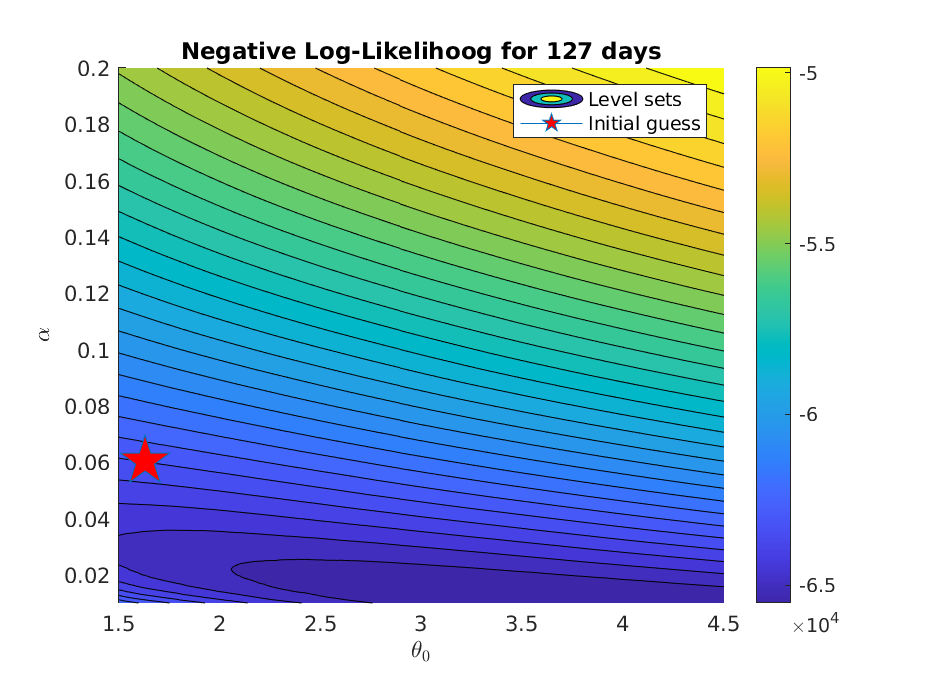
\includegraphics[width=0.32\textwidth]{../Results/likelihood/normal/Log-Likelihood_more_refined.eps}
\caption{We use the code \textbf{plotLogLikelihood.m} to create this plots. We used about 18 thousand transitions, and we can also see the initial guess.}
\end{figure}

\end{frame}


\setbeamercolor{background canvas}{bg=white!10}
\begin{frame}\frametitle{Summing-up:}

\begin{enumerate}

\item Initial guess: From quadratic variation and using all the data we get $\hat{\theta}_0\times\hat{\alpha}$. Choosing some appropiate $\gamma$, from mean least squares we get $\hat{\theta}_0$, then we also get $\hat{\alpha}$.\\
Also, from mean least squares we can estimate $\epsilon^*$, using that the least squares estimator estimates $\frac{\theta_0\alpha}{\epsilon}$ for some appropriate $\epsilon$.\\
Finally, using the pair $(\hat{\theta}_0,\hat{\alpha})$, we can obtain $\hat{\eta}$ and $\hat{\delta}$.

\item Optimal parameters: Using the training data and the initial point $(\hat{\theta}_0,\hat{\alpha})$, we can find the optimal pair $(\theta_0^*,\alpha^*)$ using the MLE. With this new pair, we can find $\eta^*$ and $\delta^*$.

\end{enumerate}

\end{frame}


\setbeamercolor{background canvas}{bg=white!10}
\begin{frame}\frametitle{Values for the parameters:}

\begin{table}[]
\begin{tabular}{cccccc}
\toprule
$\hat{\theta}_0$ & $\hat{\alpha}$ & $\hat{\eta}$ & $\hat{\delta}$ & $\gamma$ & $\epsilon$ \\
\midrule
$1.63$ & $0.06$ & *not apply* & $\SI{220}{\min}$ & $0.3$ & $0.018$ \\
\bottomrule
\end{tabular}
\end{table}
$\eta^{ini}$ is not relevant here because we do not need to remove any data to find $\delta^{ini}$.
\begin{table}[]
\begin{tabular}{ccccc}
\toprule
$\theta_0^{*}$ & $\alpha^{*}$ & $\eta^{*}$ & $\delta^{*}$ \\
\midrule
$3.91$ & $0.02$ & $0.1$ & $\SI{220}{\min}$ \\
\bottomrule
\end{tabular}
\end{table}
Notice that $\hat{\delta}=\delta^*$. However, to obtain $\delta^*$ we had to remove all initial errors larger than $\eta^*$, and in this way, we reduced the variance of the initial error. This has sense since $\theta^*_0\alpha^*<\hat{\theta}_0\hat{\alpha}$.

\end{frame}


\setbeamercolor{background canvas}{bg=white!10}
\begin{frame}\frametitle{Paths and bands for optimal values (1/4):}

\begin{figure}[ht!]
\centering
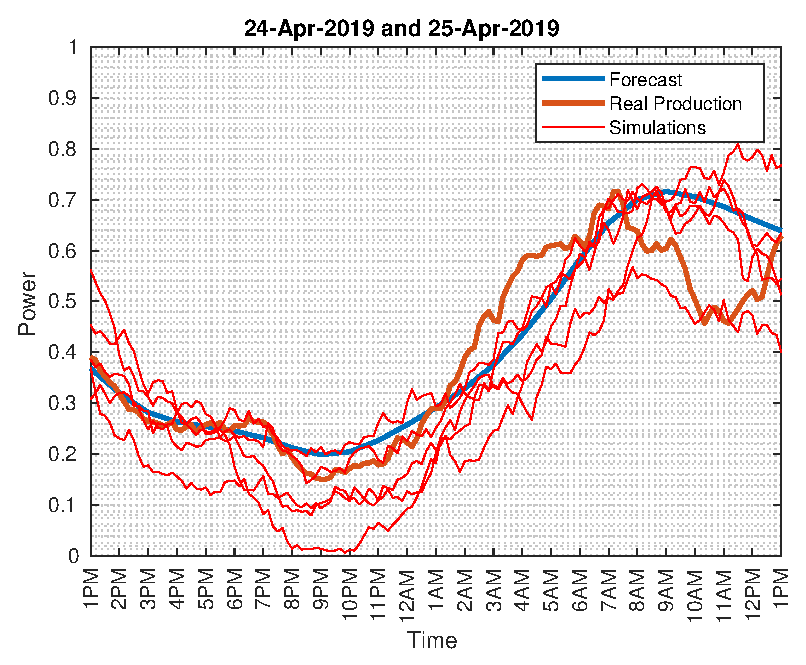
\includegraphics[width=0.4\textwidth]{../Results/paths_testing_days/optimal_value/1.eps}\quad
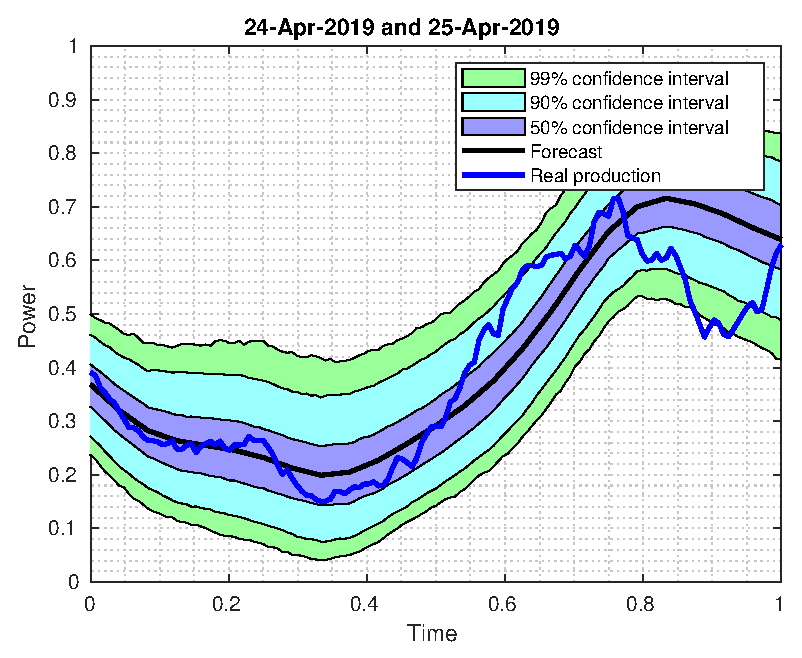
\includegraphics[width=0.4\textwidth]{../Results/bands_testing_days/optimal_value/1.eps}
\end{figure}

\end{frame}


\setbeamercolor{background canvas}{bg=white!10}
\begin{frame}\frametitle{Paths and bands for optimal values (2/4):}

\begin{figure}[ht!]
\centering
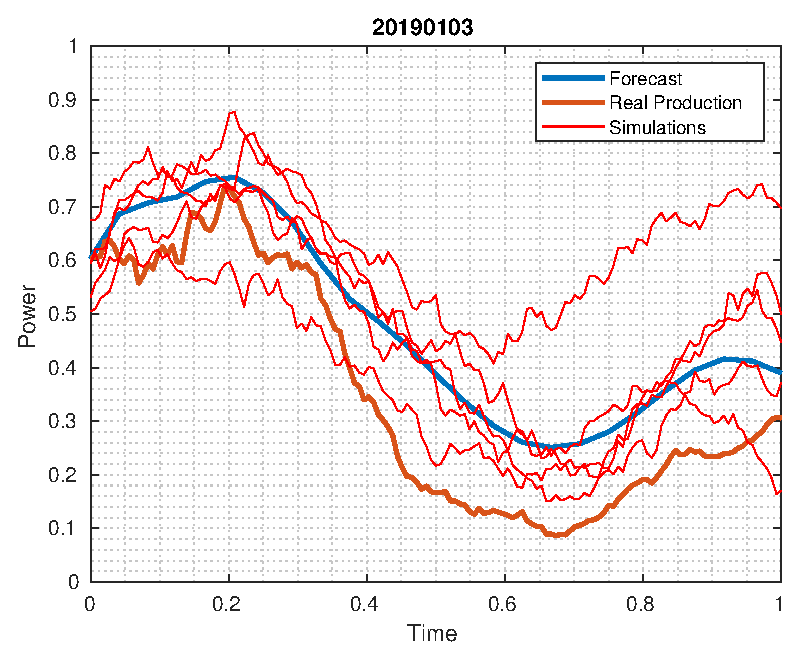
\includegraphics[width=0.4\textwidth]{../Results/paths_testing_days/optimal_value/2.eps}\quad
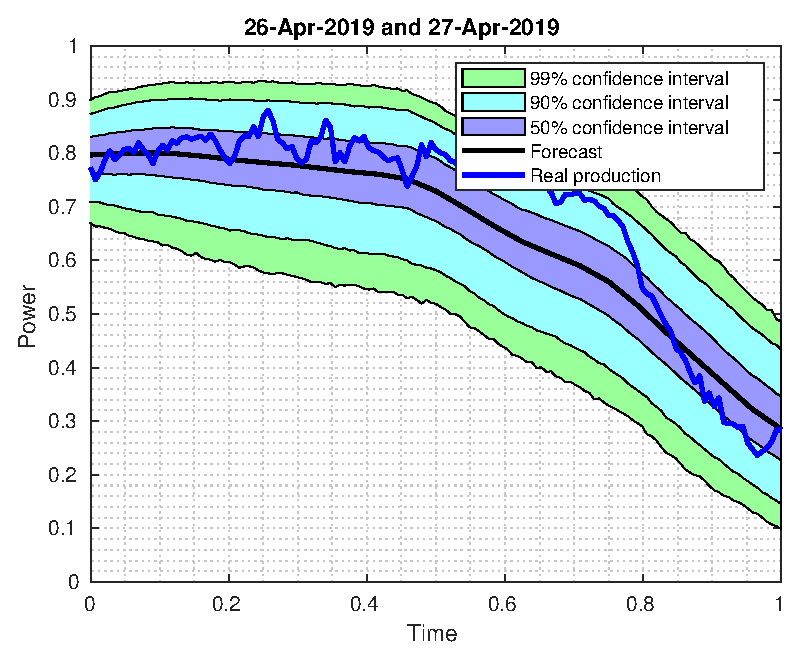
\includegraphics[width=0.4\textwidth]{../Results/bands_testing_days/optimal_value/2.eps}
\end{figure}

\end{frame}


\setbeamercolor{background canvas}{bg=white!10}
\begin{frame}\frametitle{Paths and bands for optimal values (3/4):}

\begin{figure}[ht!]
\centering
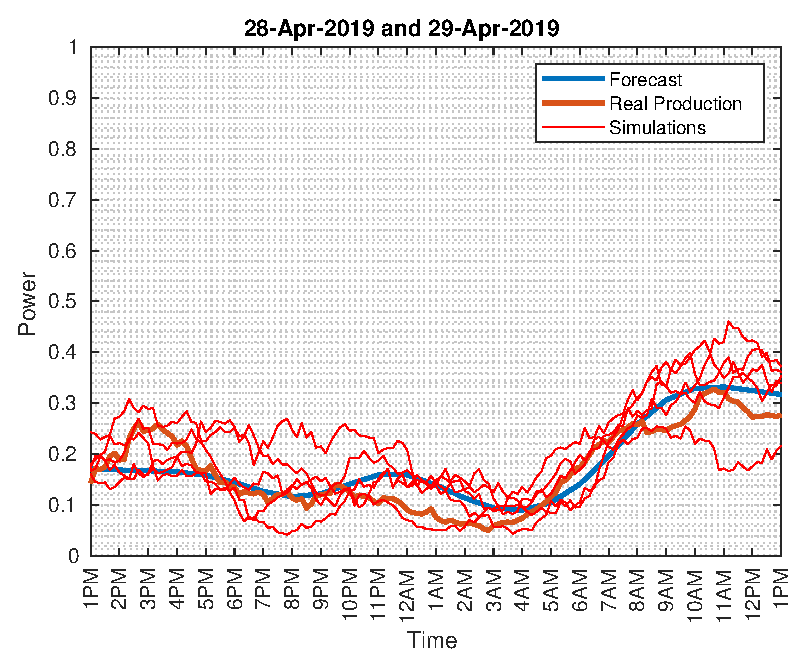
\includegraphics[width=0.4\textwidth]{../Results/paths_testing_days/optimal_value/3.eps}\quad
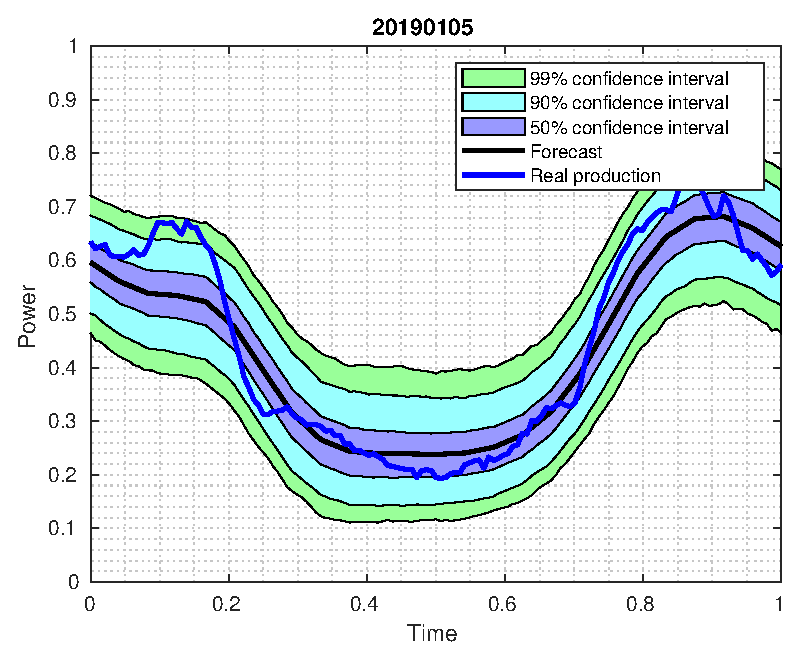
\includegraphics[width=0.4\textwidth]{../Results/bands_testing_days/optimal_value/3.eps}
\end{figure}

\end{frame}


\setbeamercolor{background canvas}{bg=white!10}
\begin{frame}\frametitle{Paths and bands for optimal values (4/4):}

\begin{figure}[ht!]
\centering
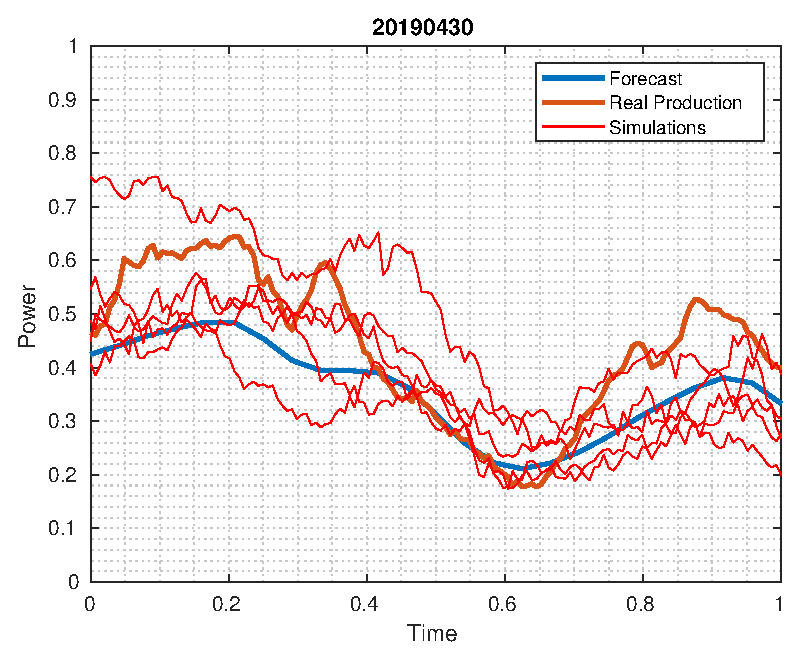
\includegraphics[width=0.4\textwidth]{../Results/paths_testing_days/optimal_value/4.eps}\quad
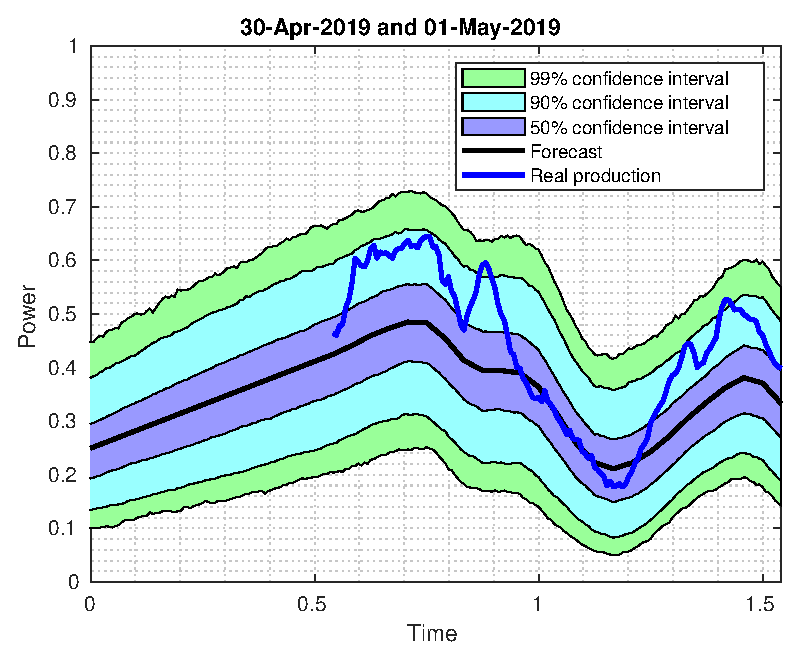
\includegraphics[width=0.4\textwidth]{../Results/bands_testing_days/optimal_value/4.eps}
\end{figure}
\end{frame}


\setbeamercolor{background canvas}{bg=green!20}
\begin{frame}

{\Huge Lamperti Transform}

\end{frame}


\setbeamercolor{background canvas}{bg=white!20}
\begin{frame}\frametitle{Two candidates:}

\begin{columns}

\column{.5\textwidth}
Recall $X_t=V_t+p_t$.\\
\quad\\
We have the candidates:
\begin{itemize}

\item {\color{blue} $Z_t=\frac{1}{\sqrt{2\alpha\theta_0}}\arcsin(2(V_t+p_t)-1)$.}
\item {\color{red} $Z_t=-\sqrt{\frac{2}{\alpha\theta_0}}\arcsin(\sqrt{1-V_t-p_t})$.}

\end{itemize}
\quad\\
\quad\\
They have the same partial derivatives. The main difference appears in the resulting SDE for $Z_t$.\\
\quad\\
For now, we will use the {\color{blue}first candidate}.

\column{.5\textwidth}
\begin{figure}[ht!]
\centering
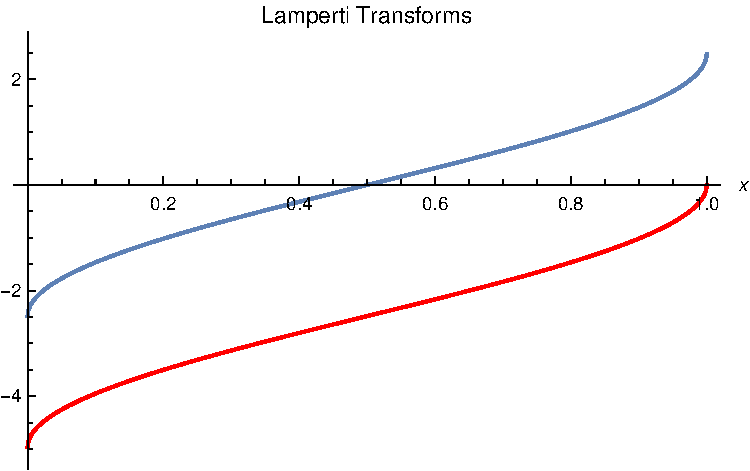
\includegraphics[width=0.9\textwidth]{../../Mathematica_Files/new_model/Lamp_Comp.pdf}
\end{figure}

\end{columns}

\end{frame}


\setbeamercolor{background canvas}{bg=white!10}
\begin{frame}\frametitle{Lamperti moments:}

The Lamperti SDE is:
\begin{align*}
\dif Z_t= \underbrace{\left[  \frac{(\alpha \theta_0 - \theta_t) {\color{black}\sin(\sqrt{2 \alpha \theta_0 } Z_t) }- \theta_t (1 - 2 p_t) + 2  \dot{p}_t }{\sqrt{2 \alpha \theta_0} \cos{(\sqrt{2 \alpha \theta_0} Z_t)}}  \right]}_{\coloneqq b(Z_t)} \dif t + \dif W_t . 
\end{align*}
Here we follow Bayesian Filtering and Smoothing, Chapter 9. We use the linearization-based approximation for the moments.\\
\quad\\
As $X_t\in(\alert{0},1)$, we have that $Z_t\in\left(\alert{-\frac{\pi}{2}\frac{1}{\sqrt{2\alpha\theta_0}}},\frac{\pi}{2}\frac{1}{\sqrt{2\alpha\theta_0}}\right)$.


\end{frame}


\setbeamercolor{background canvas}{bg=white!10}
\begin{frame}\frametitle{SDE first Lamperti moment (mean) (1/2):}
Given some measurement $z_{t_{n-1}}$, we want to compute the first moment at time $t_n$. The linearly approximated first moment $\mu_Z(s)$ for $s\in[t_{n-1},t_n]$ is the solution of the ODE

\begin{equation*}
\begin{cases}
\dif \mu_L(s)&=b(\mu_L(s))\dif s,\\
\mu_L(t_{n-1})&=z_{t_{n-1}}.
\end{cases}
\end{equation*}
\quad\\
We solve numerically the ODE using Forward-Euler:
\begin{equation*}
\mu_L(s_{n})=\mu_L(s_{n-1})+b(\mu_L(s_{n-1}))\Delta s.
\end{equation*}

\end{frame}


\setbeamercolor{background canvas}{bg=white!10}
\begin{frame}\frametitle{SDE first Lamperti moment (mean) (2/2):}

\begin{center}
\begin{tabular}{|c|}
\toprule
{\scriptsize
\lstinputlisting{../moment_1_L.m}
}\\
\bottomrule
\end{tabular}
\end{center}

\end{frame}


\setbeamercolor{background canvas}{bg=white!10}
\begin{frame}\frametitle{SDE Lamperti variance (1/2):}
Given some measurement $z_{t_{n-1}}$, we want to compute the variance at time $t_n$. The linearly approximated variance $v_Z(s)$ for $s\in[t_{n-1},t_n]$ is the solution of the ODE

\begin{equation*}
\begin{cases}
\dif \sigma^2_L(s)&=\left(2\sigma^2_Lb'(\mu_L(s))+1\right)\dif s,\\
\sigma^2_L(t_{n-1})&=0.
\end{cases}
\end{equation*}
\quad\\
We solve numerically the ODE using Forward-Euler:
\begin{equation*}
\sigma^2_L(s_{n})=\sigma^2_L(s_{n-1})+\left(1+2\sigma^2_L(s_{n-1})b'(\mu_L(s_{n-1}))\right)\Delta s.
\end{equation*}
We have that (computed with Mathematica):
\begin{equation*}
b'(z)=\frac{\dif b}{\dif z}(z)=\frac{\alpha\theta_0-\theta_t+(2\dot{p}_t+(2p_t-1)\theta_t)\sin(z\sqrt{2\alpha\theta_0}))}{\cos^2(z\sqrt{2\alpha\theta_0})}.
\end{equation*}

\end{frame}


\setbeamercolor{background canvas}{bg=white!10}
\begin{frame}\frametitle{SDE Lamperti variance (2/2):}

\begin{center}
\begin{tabular}{|c|}
\toprule
{\tiny
\lstinputlisting{../moment_2_L.m}
}\\
\bottomrule
\end{tabular}
\end{center}

\end{frame}


\setbeamercolor{background canvas}{bg=white!10}
\begin{frame}\frametitle{Density next measurement:}

We want the next measurement $Z_{t_n}|Z_{t_{n-1}}$ to have a Gaussian with mean $\mu_Z$ and variance $\sigma_Z^2$ ($f_Z(z)=\mathcal{N}(\mu_Z,\sigma^2_Z)$).\\
\quad\\
Then, we want the SDE and our new PDF $f_Z(z)$ to have the same moments at each $t\in\{\text{some appropriate domain}\}$, i.e., $\mu_Z(t)=\mu_L(t)$ and $\sigma^2_Z(t)=\sigma^2_L(t)$.\\
\quad\\
The density and log-density (natural logarithm) are:
\begin{equation*}
f_Z(z)=\frac{e^{-\frac{1}{2}\left(\frac{z-\mu_Z}{\sigma_Z}\right)^2}}{\sigma_Z\sqrt{2\pi}}\iff \log(f_Z(z))=-\frac{1}{2}\left(\frac{z-\mu_Z}{\sigma_Z}\right)^2-\log(\sigma_Z\sqrt{2\pi}).
\end{equation*}

\begin{center}
\begin{tabular}{|c|}
\toprule
{\tiny
\lstinputlisting{../log_dist_L.m}
}\\
\bottomrule
\end{tabular}
\end{center}

\end{frame}


\setbeamercolor{background canvas}{bg=white!10}
\begin{frame}\frametitle{Lamperti Log-likelihood evaluation (1/2): CODE}

\begin{center}
\begin{tabular}{|c|}
\toprule
{\tiny
\lstinputlisting{../log_LH_evaluation_L.m}
}\\
\bottomrule
\end{tabular}
\end{center}

\end{frame}


\setbeamercolor{background canvas}{bg=white!10}
\begin{frame}\frametitle{Lamperti Log-likelihood evaluation (2/2):}

\begin{figure}[ht!]
\centering
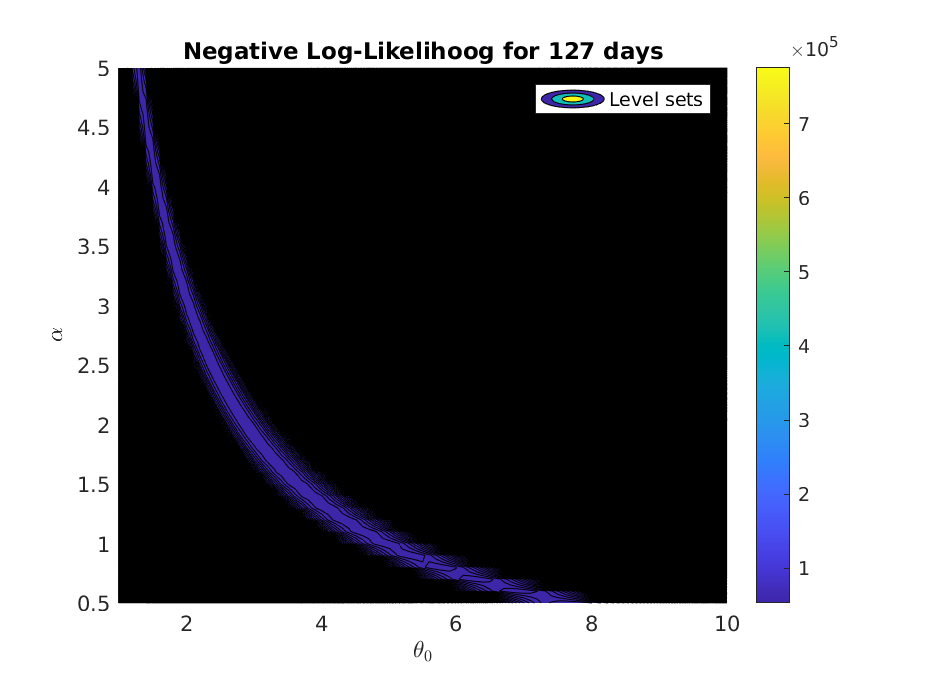
\includegraphics[width=0.5\textwidth]{../Results/likelihood/lamperti/Log-Likelihood.eps}
\caption{We use the code \textbf{plotLogLikelihood.m} to create this plots. We used about 18 thousand transitions.}
\end{figure}

\end{frame}


\end{document}